% Compile after running scripts/paper_tables.py.
\documentclass[conference]{IEEEtran}
\usepackage{booktabs,amsmath,graphicx,url}
\usepackage[hidelinks]{hyperref}
\newcommand{\NewAttempts}{620}
\newcommand{\TotalAttempts}{992}
\newcommand{\ReviewEligible}{804}
\newcommand{\ReviewSample}{161}
\newcommand{\BreadthAttempts}{400}
\newcommand{\PanelRows}{DeepSeek Coder 1.3B & 5/12 & 5/12 & 2/12 & 2/12 \\
GPT-5.4 nano & 8/12 & 8/12 & 8/12 & 8/12 \\
DeepSeek V4 Flash & 6/7 & 6/7 & 6/7 & 6/7 \\
Qwen2.5-Coder 1.5B & 5/12 & 5/12 & 7/12 & 6/12 \\
SmolLM2 1.7B & 2/12 & 5/12 & 4/12 & 4/12 \\}
\newcommand{\ProbeRows}{DeepSeek Coder 1.3B & QuixBugs & 12 & 3 & 3 \\
DeepSeek Coder 1.3B & ConDefects & 12 & 0 & 0 \\
GPT-5.4 nano & QuixBugs & 12 & 0 & 0 \\
GPT-5.4 nano & ConDefects & 12 & 0 & 0 \\
Qwen2.5-Coder 1.5B & QuixBugs & 12 & 4 & 0 \\
Qwen2.5-Coder 1.5B & ConDefects & 12 & 1 & 0 \\
SmolLM2 1.7B & QuixBugs & 12 & 5 & 2 \\
SmolLM2 1.7B & ConDefects & 12 & 0 & 0 \\}
\newcommand{\BreadthRows}{S0 & 100 & 66 & 5 & 29 & 1.00 \\
S1 & 100 & 80 & 7 & 13 & 1.52 \\
S2 & 100 & 71 & 5 & 24 & 3.60 \\
S2-R & 100 & 73 & 5 & 22 & 2.54 \\}
\newcommand{\WidePairs}{S1 & S2 & 100 & 16 & 7 & 0.093 \\
S2 & S2-R & 100 & 7 & 9 & 0.804 \\}

\newcommand{\FullModelRows}{%
QuixBugs & GPT-5.4 nano & 28 & 27 & 29 & 27\\
QuixBugs & Qwen Coder & 11 & 11 & 9 & 10\\
QuixBugs & SmolLM2 & 7 & 9 & 16 & 12\\
ConDefects & GPT-5.4 nano & 66 & 80 & 71 & 73\\
ConDefects & Qwen Coder & 8 & 8 & 5 & 7\\
ConDefects & SmolLM2 & 3 & 4 & 9 & 5\\%
}

\newcommand{\AdditionalModelRows}{%
QuixBugs & GPT-4o mini & 23/31 & 27/31 & 25/31 & 22/31\\
QuixBugs & GPT-4.1 mini & 28/31 & 28/31 & 27/31 & 27/31\\
QuixBugs & OLMo 2 1B & 0/2 & 0/3 & 0/2 & 0/2\\
QuixBugs & Granite 3.3 2B & -- & -- & -- & --\\
QuixBugs & Phi-3 mini & -- & -- & -- & --\\
ConDefects & GPT-4o mini & 62/100 & 68/100 & 61/100 & 65/100\\
ConDefects & GPT-4.1 mini & 74/100 & 79/100 & 75/100 & 77/100\\
ConDefects & OLMo 2 1B & 0/23 & 0/23 & 0/23 & 0/23\\
ConDefects & Granite 3.3 2B & -- & -- & -- & --\\
ConDefects & Phi-3 mini & -- & -- & -- & --\\%
}

\title{When a Code Reviewer Agrees with a Wrong Patch:\\Budget-Controlled Language-Model Repair on Python Bugs}
\author{\IEEEauthorblockN{SW403 project research draft for team review}
\IEEEauthorblockA{AI in Modern Software Engineering, Zewail City of Science and Technology\\
Fall 2026 \quad$\cdot$\quad AI assistance and outstanding human review are disclosed in Section~\ref{sec:ethics}}}
\begin{document}
\maketitle
\begin{abstract}
A repair workflow can spend extra model calls on diagnosis, retries or review. We study which use of those calls yields patches that survive additional tests. The starting evidence is a frozen set of 372 Gemini 3.5 Flash-Lite attempts on 31 QuixBugs programs. The initial Phase~3 collection contains \NewAttempts{} observed attempts, including a matched identifier-renaming panel and a difficulty-stratified ConDefects evaluation. Subsequent full-dataset trials and a separate browser study extend that collection. Each repair sees the original source and failing examples. We evaluate its final candidate on a second test partition. The archived single agent passed both partitions in 90 of 93 attempts. The agent team passed in 89, while using 3.2 times as many output tokens per attempt. Two of its approvals endorsed a patch that mishandled all-negative lists. On 100 distinct ConDefects tasks, GPT-5.4 nano repaired 80 with the single agent and 71 with the agent team (paired exact $p=0.093$). In the new matched panel, GPT-5.4 nano reproduced that error after renaming. We report paired counts, model-specific budgets and trace-level counterexamples. A reviewer that shares the fixer's assumptions can miss exactly the distinction that a held-out test exposes.
\end{abstract}
\begin{IEEEkeywords}
automated program repair, multi-agent systems, test-suite overfitting, software engineering, large language models
\end{IEEEkeywords}

\section{Introduction and Problem Definition}
A faulty program can be only one line away from two very different repairs. Consider a function that returns the maximum sum of a contiguous slice. If the empty slice is admissible, an all-negative input must return zero. If at least one element is required, the same input must return its largest element. Both interpretations admit the same implementation on many ordinary examples. In our trace, an agent repaired the function according to the second convention. A reviewer cited the handling of negative values as its reason for approval. A single held-out example distinguished the two contracts.

A team can spend one call locating a fault, a second writing code and a third reviewing the result. A single agent can spend the same allowance on successive patches with interpreter feedback. We hold the ceiling constant and record how many calls each workflow actually uses.

The study asks three questions.
\begin{enumerate}
\item Under a common call and output-token ceiling, how often does each architecture repair the same bugs?
\item What does a reviewer contribute after the candidate has already passed the visible tests? How often does its decision agree with the reserved tests?
\item When the same function and examples appear under unfamiliar identifiers, which outcomes change? Does that pattern differ between datasets?
\end{enumerate}
The primary outcome is an attempt that passes both test partitions. The evaluator stores the partitions' results separately so that another researcher can distinguish an immediately detectable failure from an overfit patch. The archived study, the paired small panel and the broader contest sample have different denominators and support different claims.

\section{Related Work}
QuixBugs packages small algorithmic defects with repaired versions~\cite{quix}. It makes repair experiments inexpensive and failures easy to inspect. Its longevity also gives a model opportunities to encounter its names, algorithms and tests during training. Hu et al.\ reported repairing all 40 QuixBugs programs with GPT-o1 in their protocol~\cite{hu}. Their result illustrates how little headroom an aggregate success rate may leave on this benchmark. Our archived sample uses 31 functions with JSON test data, a particular visible/held-out split and repeated attempts. Comparing the two percentages requires aligning the evaluation choices.

ConDefects complements small textbook algorithms with programs submitted to competitive-programming tasks. Wu et al.\ motivated their dataset by the ability to select faults by date and difficulty~\cite{wu}. Its records provide a faulty submission and a corresponding repaired program. A historical date can constrain what an earlier model could have seen. For a model released years later, both the contest and the repair corpus may already have been public. We use ConDefects to broaden the population of programs and retain its publication history as provenance.

The generate-and-validate literature distinguishes satisfying the available test suite from implementing the intended behavior~\cite{qi}. This distinction becomes particularly important when an agent receives test feedback several times. Iteration increases the opportunity to discover a repair, but it also provides repeated access to the same finite set of examples. Chen et al.\ studied how a language model can use execution and explanations to debug its own programs~\cite{chen}. Our feedback baseline isolates one version of that mechanism. It repeats only after a candidate fails a visible test, so easy cases never exercise a second turn.

Cemri et al.\ describe multi-agent failures involving coordination, task specification and verification~\cite{mast}. We use these broad categories to interpret trace sequences. The evaluator's five automatic indicators describe observable properties of a patch or verdict. Interpreting a sequence as a coordination failure requires reading what one role communicated to the next. The trace analysis and the automated indicators answer different questions.

\section{Systems and Measurements}
\subsection{Information available to each agent}
A bug record contains source code, a callable entry point, visible examples, a reserved set of examples and a reference program. Only the evaluator and dataset checks use the final two fields. The initial tool call runs the faulty code on the visible examples. The prompt includes the program, expected outputs and an execution summary. Every workflow therefore starts with evidence that the original is faulty. Later turns can see feedback generated within the same attempt. A fresh attempt starts from the original source.

S0 makes one request for a replacement program. S1 starts with the same repair request and returns interpreter failures to the model when a candidate fails a visible example. S2 begins with a localiser that receives numbered source and explains the likely fault. The fixer receives the program, the visible evidence and the localisation. A deterministic tool tests the proposed program. A failure returns control to the fixer. A visible pass sends the candidate to a reviewer. A rejection supplies feedback for another fix when budget remains. S2-R removes the reviewer and returns the first visible-passing candidate. The roles use separate conversations with the same base model.

The multi-agent implementation retains its latest visible-passing candidate so an exhausted retry cannot silently discard it. The recorded verdict belongs to that candidate. If the final candidate has yet to be reviewed, its verdict is missing. Counting a missing verdict as a rejection would overstate the number of bad patches caught. The number of rejection messages in the trace and the number of final candidates rejected also have different denominators.

\subsection{The unit of comparison}
One unit is a bug variant, system, model and run index. A run terminates at a system-specific stop condition or exhaustion of the shared allowance. The archived Gemini ceiling is eight completed requests and 8,000 output tokens per attempt. The new experiments use four requests and 1,536 output tokens, with at most 512 per call. Temperature is requested at 0.2. The new limits leave room for one complete localise--fix--review path and a further action. They can truncate a long program, particularly in the broader contest sample. We preserve the limit across architectures within each block. S0 can consume only its first call, even when allowance remains.

A call ceiling measures available resources. The log measures consumption. We record prompt tokens, completion tokens, calls and wall time. An S2 fixer receives a localisation and sometimes several feedback summaries. A later prompt can therefore cost more than a first request even if both generate equally long code. Token counts are provider-specific, and wall time includes service latency and test execution. The replication package records model aliases and checksums for the local quantized weights.

\subsection{Labels and statistical analysis}
A final program that passes both partitions receives the operational label \emph{correct}. Passing the visible examples and failing a reserved example produces \emph{plausible-incorrect}. A visible failure produces \emph{failing}, irrespective of how many reserved examples pass. The overfitting denominator consists of final programs that pass the visible suite. This distinction matters when comparing a system that produces many visibly invalid programs with one that overfits its examples.

We flag code that cannot load (H1), unresolved names or newly introduced third-party imports (H2), changes to recorded top-level parameter names (H3), an AST-equivalent final program (H4), and reviewer approval followed by a failed evaluation (H5). Flags can overlap. An unresolved name can result from a typo. A changed parameter name may still work for every positional call. H4 may arise when a system returns the original source at exhaustion. Flag totals therefore measure specific signals and require interpretation alongside the test outcomes.

For two systems, let $b$ count units solved only by the first and $c$ units solved only by the second. Exact McNemar uses a two-sided binomial test on the $b+c$ discordant pairs. Concordant pairs affect the rates but supply no evidence for directional asymmetry. The effect in percentage points is $100(c-b)/n$. Archived confidence intervals resample whole bugs, preserving their repeated runs. The archive's paired tests use bug--run pairs, which may remain correlated within a bug. The broader sample has one run per system per task. On the small panel, cross-system totals for renaming are descriptive because the four observations of a function share cases.


\section{Datasets and Prototype}
\subsection{An archived block and two new designs}
The archive contains 31 QuixBugs programs, four systems and three runs for each combination. It contains 118 visible and 122 reserved examples across the 31 bugs. The dataset preparation excluded the nine graph programs that use node objects, removed slow examples already skipped upstream and used a fixed split. We analyze the saved attempts from the study model \texttt{gemini-3.5-flash-lite}. Reusing these records preserves the observed traces and their original budget.

The matched panel asks a narrower question under a controlled intervention. It includes greatest common divisor, balanced parentheses and maximum sublist sum, plus three ConDefects submissions covering positive multiples of 100, cyclic string rotations and distinct permutations of three characters. This purposive choice includes a recurrent archived failure and programs with different control flow. We create an original and a renamed version of each. The six subjects are the independent program identities. Twelve presentations of source code and four architectures yield 48 attempts per completed model panel.

For the three contest programs, a mechanical adapter turns a single input line into an argument and printed lines into a returned string. The test oracles follow the task operations independently of the submitted repair. They check positivity and divisibility, enumerate cyclic rotations or count distinct permutations. The renamed copy changes the function name, parameters and stored identifiers at token boundaries, including recursive calls. It preserves literals, comments and prose. We run the reference and defective versions with the same inputs and require the same failing case IDs before acceptance. Descriptive text can still identify a familiar algorithm. The intervention estimates identifier sensitivity under that constraint.

The breadth experiment takes one Python submission per AtCoder task from the pinned ConDefects snapshot. The allocation is 60 tasks with difficulty 0--399, 30 with 400--1199 and ten with 1200 or higher. Within each band, the builder shuffles tasks and candidate submissions with a recorded seed. Eligibility requires at least two distinct public input examples, code and examples short enough for the prompt, a reference that passes the examples and a faulty version that fails a visible example. Tasks from the small contest panel are excluded. The split reserves failing examples on both sides whenever the available cases permit it. Each record links the submission source and public example page.

This design favors bugs detectable through public examples. It excludes some faults that emerge only on the private contest judge and some long, dependency-heavy programs. A reference's success validates the adapter on the selected inputs. A random sample from the whole corpus would answer a different question. Our breadth results describe the selected 100 tasks under this particular oracle.

\subsection{Execution and replication}
The code, datasets, run traces, analysis scripts and recorded demo are available at \url{https://github.com/seif-356/AI_modern_software/tree/phase-3-study}.

The prototype exposes a FastAPI repair endpoint, an experiment runner, an evaluator and a Streamlit trace viewer. The repair endpoint accepts submitted Python, positional examples and a system choice. The runner records the model, dataset digest, budget, trace, final code and outcomes. It writes each completed attempt as JSONL, so a provider interruption can be resumed. A dry run inspects remaining work without contacting a model. A separate replay script executes an archived candidate and prints the reserved example that refutes its review.

Candidate code runs in a temporary working directory under an isolated Python interpreter. The child receives a restricted environment. On POSIX the harness uses interval timers and attempts an address-space limit. On Windows the parent enforces a wall timeout per case using separate processes. These mechanisms support the controlled benchmark workflow. A public service accepting arbitrary submissions would also need operating-system isolation and resource controls outside the Python process. The course demo runs locally on benchmark data.

\section{Evaluation and Results}
Across 100 distinct contest tasks with GPT-5.4 nano, S1 produced 80 test-correct candidates and S2 produced 71. This nine-point observed difference was accompanied by a 2.4-fold increase in mean calls for S2. The paired test below quantifies the uncertainty. The archived and matched-panel results first show how the contrast changes when the programs and models change.
\subsection{Archived Gemini evidence}
\begin{table}[ht]
\caption{Archived QuixBugs outcomes and mean usage. Each row has 93 attempts. Wrong denotes a visible pass that failed held-out tests.}
\centering\footnotesize
\begin{tabular}{lrrrrr}\toprule
System & Correct & Wrong & Failing & Calls & Out tokens\\\midrule
S0 &90&3&0&1.00&107\\
S1 &90&3&0&1.00&106\\
S2 &89&2&2&3.76&341\\
S2-R &88&3&2&2.19&198\\\bottomrule
\end{tabular}
\end{table}
Every S0 and S1 first patch passed the visible suite. Consequently S1 consumed exactly one call throughout this block. S1's bug-bootstrap 95\% interval is 0.903--1.000. The corresponding interval for S2 is 0.892--1.000. In the direct pairing, two units favor S1 and one favors S2, giving an exact $p=1.0$. Equal success on most units and few discordant pairs make this an imprecise comparison. These data support a cost observation more readily than an accuracy ordering.

The reviewer issued decisions on 84 final S2 patches. It approved 81 that passed all tests and two that failed the reserved suite, and rejected one that passed. Approval precision is $81/83$, while the catch rate among the two observed wrong reviewed patches is $0/2$. High approval precision is compatible with little discriminative value when almost every candidate reaching review already works. The other nine attempts lack an applicable final review in this accounting.

\subsection{New model panels and renaming}
\begin{table}[ht]
\caption{Correct attempts per recorded attempt on the matched panel, original and renamed combined. Each system has 12 planned attempts per model.}
\centering\scriptsize
\begin{tabular}{lrrrr}\toprule Model & S0 & S1 & S2 & S2-R\\\midrule
\PanelRows
\bottomrule\end{tabular}
\end{table}
Each numerator counts attempts whose final patch passes both partitions. Each denominator counts records in that system's run file. Within each row the same base model supplies all roles. Local models use pinned four-bit weights. GPT is a dated hosted snapshot.

Across the matched panel and breadth study, the 448 GPT attempts used 551,202 input tokens and 210,299 output tokens, an estimated US\$0.37 at the listed uncached rates. The two local models incurred no provider API fees. Meta's API declined generation during billing verification. We evaluated its consumer web app separately.

GPT fixed two of the three original QuixBugs programs under each architecture, and the same two after renaming. The failed maximum-sublist case generalizes the archived reviewer example to another model under a smaller budget. In the contest subset GPT also fixed two of three originals and two of three renamed programs under every architecture. The totals conceal a change in failure type. An S1 original that accepted only 100 passed visible tests and failed a reserved larger multiple. Its renamed counterpart failed visible tests. Binary correctness alone misses that difference.

\begin{table}[ht]
\caption{Renaming discordances. Counts pool the four systems descriptively within each dataset. $O$ and $R$ denote original-only and renamed-only successes.}
\centering\scriptsize
\begin{tabular}{llrrr}\toprule Model & Dataset & Pairs & $O$ & $R$\\\midrule
\ProbeRows
\bottomrule\end{tabular}
\end{table}
Stability after renaming can reflect robust reasoning, a recognizable specification or knowledge of a familiar algorithm. A change can reflect sampling variation or identifier sensitivity. A single generation per condition cannot distinguish these explanations.

\subsection{Breadth across contest tasks}
\begin{table}[ht]
\caption{GPT-5.4 nano on the difficulty-stratified ConDefects sample. Each submitted program is a distinct task.}
\centering\footnotesize
\begin{tabular}{lrrrrr}\toprule System & Attempts & Correct & Wrong & Failing & Calls\\\midrule
\BreadthRows
\bottomrule\end{tabular}
\end{table}
The breadth study has \BreadthAttempts{} completed attempts. Each agent repairs a string-to-string function using code and visible examples. Using public example outputs admits more tasks, but leaves some with only one reserved example.

\begin{table}[ht]
\caption{Exact paired breadth comparisons. Columns A only and B only give the discordant task counts.}
\centering\footnotesize
\begin{tabular}{llrrrr}\toprule A & B & Paired & A only & B only & $p$\\\midrule
\WidePairs
\bottomrule\end{tabular}
\end{table}
The paired counts show how often switching systems changes the outcome on the same task. The tables also distinguish visible failures from patches that pass visible tests but fail reserved examples.


S1 alone repaired 16 tasks that S2 missed, while S2 alone repaired seven. The exact two-sided $p$-value is 0.093. This sample favors the single-agent feedback loop descriptively, but the comparison does not establish a population-level advantage at the conventional 0.05 threshold. Removing the reviewer from S2 changed 16 paired outcomes: seven favored S2 and nine favored S2-R ($p=0.804$). S1 spent 1.52 calls and 469 output tokens per task. S2 spent 3.60 calls and 718 tokens. Among the 48 final S2 reviews, 39 approved correct patches, two approved wrong patches, six rejected correct patches and one rejected a wrong patch. The other 52 final candidates had no applicable verdict.

\begin{figure}[ht]
\centering
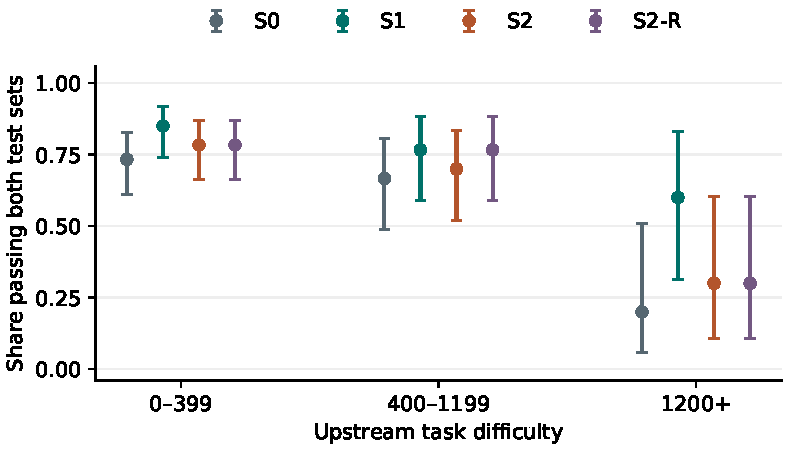
\includegraphics[width=\columnwidth]{../../results/phase3/figures/difficulty.pdf}
\caption{Correctness by ConDefects task difficulty on the GPT breadth run. Each point uses a different set of 60, 30 or 10 tasks across bands and the same tasks within a band. Bars show 95\% Wilson intervals.}
\end{figure}

\subsection{How the broader sample tests the reviewer}
One GPT S2 trace illustrates why reserved examples remain valuable even when reviewing a plausible patch on a fresh task. In AtCoder ABC235 B the program should follow the initial strictly increasing sequence of heights and stop as soon as the next height does not rise. The single visible sequence, $(1,5,10,4,2)$, reaches its global maximum at that stopping point. The fixer replaced the loop with a global maximum calculation. The reviewer approved the change and described the old early exit as the cause of the failure. Both algorithms return 10 for the visible input.

The reserved sequence $(27,1828,1828,9242)$ makes the difference observable. A hiker following the rule stops at the plateau and reports 1828. The generated program continues to the distant peak and reports 9242. A second reserved sequence that rises throughout also passes the global-maximum implementation. The verdict therefore turns on the placement of one plateau. Finding more tests of the increasing sequence alone would not resolve the ambiguity. The example also supplies the team with a concrete adjudication rationale for a hypothetical patch with the same behavior.

The broader split has 137 visible examples and 144 reserved examples over 100 submissions. With so few cases per task, one example can dominate both the repair decision and the evaluation. The difficulty bands partly address population diversity. They do not increase the number of examples for a given specification. The top band contains only ten tasks, so its interval is especially sensitive to a single outcome. Apparent differences between adjacent points in the figure should be checked against the underlying paired discordances.

\subsection{Supplementary Muse web-app panel}
We ran all four workflows on the same six programs, each in its original and renamed form, through the Muse web app in Edge. Each role received its prompt in a new side chat. The first GCD pilot supplied its prespecified S0 cell. We used 84 browser submissions across the 48 scored attempts. Before scoring the final panel, we discarded a collection pass with 27 saved replies after finding that some displayed code blocks were incomplete. We then captured complete patches using the site's copy control. The app's model version, internal calls, temperature, token usage and account memory were uncontrolled. We therefore report this panel separately from the 992-attempt study.

\begin{table}[ht]
\centering
\caption{Supplementary Muse browser panel. Each workflow saw the same 12 variants. Submissions count messages sent by the experimenter.}
\begin{tabular}{lrrr}\toprule
Workflow & Visible pass & Held-out pass & Submissions\\\midrule
S0   & 12 & 10 & 12\\
S1   & 12 & 10 & 12\\
S2   & 12 & 10 & 36\\
S2-R & 12 & 10 & 24\\\bottomrule
\end{tabular}
\end{table}
All four workflows repaired the same 10 variants. All eight held-out failures came from the original and renamed versions of one contest task, ABC223 A. On both presentations, the S2 reviewer approved a patch that accepted exactly 100. The reserved examples required positive multiples such as 200 and 500 to pass as well. On these six programs, spending additional submissions on localisation and review did not change which variants passed.

\subsection{Muse browser results on the full datasets}
We evaluated one attempt per workflow on each of the 31 original QuixBugs programs and 100 distinct ConDefects tasks. The 524 cells represent 131 subjects. Three QuixBugs inputs matched the earlier browser panel in every field. We reused and rescored their 12 workflow results (21 messages). The other 512 cells used 902 newly captured messages in Edge. We excluded 27 first-pass trials after a capture audit found 34 missing code blocks and repeated those trials in full. The 63 replies from the excluded trials do not enter the table.

\begin{table}[ht]
\centering
\caption{Full Muse browser sample. Visible and Both count tasks passing the visible tests and both partitions, respectively. Msgs counts messages contributing to the scored trials.}
\label{tab:muse-full}
\begin{tabular}{lrrrrrr}\toprule
& \multicolumn{3}{c}{QuixBugs ($n=31$)} & \multicolumn{3}{c}{ConDefects ($n=100$)}\\
\cmidrule(lr){2-4}\cmidrule(lr){5-7}
Workflow & Visible & Both & Msgs & Visible & Both & Msgs\\\midrule
S0   & 31 & 30 & 31 & 98 & 96 & 100\\
S1   & 31 & 30 & 31 & 100 & 97 & 102\\
S2   & 31 & 30 & 94 & 100 & 98 & 303\\
S2-R & 31 & 30 & 62 & 100 & 98 & 200\\\bottomrule
\end{tabular}
\end{table}

All four browser workflows passed the same 30 of 31 QuixBugs programs. Each timed out on one held-out Levenshtein case during collection. The S0 patch passed that case on a subsequent local execution, so this result depends on runtime. On ConDefects, S2 and S2-R tied for the highest pass count, repairing the same 98 of 100 tasks. Both missed ABC354 A and ABC285 A despite passing every visible example. Adding the reviewer produced no additional passing tasks on either dataset. On ConDefects the reviewed team used 303 browser messages, compared with 200 for the reviewer-free team. The browser exposed neither the underlying model version nor its token budget.

\subsection{Full-dataset extension for GPT and local models}
We applied the four workflows once to each original QuixBugs program and each breadth-sample ConDefects task using GPT-5.4 nano, Qwen2.5-Coder 1.5B and SmolLM2 1.7B. Each model already had 12 workflow results on three identical QuixBugs inputs. GPT also had all 400 ConDefects results. These 436 earlier observations and 1,136 newly scored trials cover all 1,572 combinations. The Muse browser product and the Gemini archive have separate measurement protocols.

\begin{table}[ht]
\centering
\caption{Tasks passing both test partitions. Each workflow saw all 31 original QuixBugs programs or all 100 ConDefects tasks.}
\label{tab:full-models}
\begin{tabular}{llrrrr}\toprule
Dataset & Model & S0 & S1 & S2 & S2-R\\\midrule
\FullModelRows
\bottomrule\end{tabular}
\end{table}

On ConDefects, moving from S1 to S2 changed the pass counts from 80 to 71 for GPT, 8 to 5 for Qwen, and 4 to 9 for SmolLM2. The direction of the change depended on the model. These counts describe one trial per cell on the selected tasks.

The local models used the same pinned quantized weights as the matched panel. Six new QuixBugs trials on \texttt{wrap} stopped when a later prompt reached the input byte limit or the local context limit. The scorer evaluated the candidate available at that point. All six stops are identified in the raw records.



\subsection{Additional hosted and local models}
We extended the same four workflows to two dated OpenAI snapshots (GPT-4o mini and GPT-4.1 mini) and three local four-bit instruction models (OLMo 2 1B, Granite 3.3 2B, and Phi-3 mini). The dataset, test partitions, temperature and per-attempt ceilings match the full-dataset extension. Each model has 124 planned QuixBugs trials and 400 planned ConDefects trials. A shared \$1.50 ceiling covers both hosted models. The runner reserves the maximum estimated cost before each request and reconciles it against reported tokens at standard uncached rates. The local runs incur no API fee.

\begin{table}[ht]
\centering\small
\setlength{\tabcolsep}{3pt}
\caption{Additional models. Each entry gives repairs passing both test partitions divided by completed trials. A dash denotes zero completed trials. Each workflow has 31 planned QuixBugs trials and 100 planned ConDefects trials.}
\label{tab:additional-models}
\begin{tabular}{@{}llrrrr@{}}\toprule
Dataset & Model & S0 & S1 & S2 & S2-R\\\midrule
\AdditionalModelRows
\bottomrule\end{tabular}
\end{table}

Both additional GPT models completed all 524 planned trials. On ConDefects, single-agent retry (S1) passed 79 tasks with GPT-4.1 mini and 68 with GPT-4o mini. The agent team (S2) passed 75 and 61, respectively. The same workflow ordering held on QuixBugs. These counts describe one trial per workflow and task. Reported tokens across the hosted extension cost \$0.7951 at uncached rates. Eight requests without confirmed usage retained \$0.0076 in reservations, giving a conservative combined bound of \$0.8027.

\subsection{Workflow performance across the eight complete models}
We counted one trial per workflow for each model and task in Tables~\ref{tab:full-models} and~\ref{tab:additional-models}. Each model received equal weight. Table~\ref{tab:workflow-comparison} reports the number of trials passing both test partitions. On QuixBugs the reviewed team (S2) led with 140 of 248 passes (56.5\%). On ConDefects the single agent with test feedback (S1) led with 280 of 800 (35.0\%), passing 40 more model--task pairs than S2.

\begin{table}[ht]
\centering\small
\caption{Pass counts across eight models. The denominator for each workflow is eight models times the number of tasks in that dataset. Bold marks the highest observed count.}
\label{tab:workflow-comparison}
\begin{tabular}{lrrrrr}\toprule
Dataset & Trials/workflow & S0 & S1 & S2 & S2-R\\\midrule
QuixBugs & 248 & 125 & 134 & \textbf{140} & 135\\
ConDefects & 800 & 238 & \textbf{280} & 240 & 252\\\bottomrule
\end{tabular}
\end{table}

We paired the reviewed and reviewer-free outcomes on the same model and task. On QuixBugs, 14 pairs passed only with review and nine passed only without it, a net gain of five passes (2.0 percentage points). On ConDefects, 27 pairs passed only with review and 39 passed only without it, a net loss of 12 passes (1.5 percentage points). Each workflow generated its own candidate once per pair. The comparison therefore measures the outcome of the whole workflow and cannot isolate the effect of a reviewer decision on a fixed candidate.

\section{Discussion}
\subsection{Where extra calls go}
The agent team commits a call to localisation before it tests a fix. That cost is certain even when the defect is obvious. Its benefit depends on whether the diagnosis draws attention to evidence the fixer would have missed. The same dependency can lead a fixer away from the fault. In the archived \texttt{wrap} trace, the localiser focused on whitespace between lines. The fixer appended a final line, but also altered how spaces were carried into the following line. Subsequent fixes kept modifying the split. The visible tests detected the problem, yet repeated feedback did not dislodge the initial diagnosis. This sequence is consistent with inter-agent misalignment in MAST. A counterfactual run with only the diagnosis changed would be needed to attribute causation.

The maximum-sublist trace illustrates a different mechanism. A textbook implementation initializes the running sum to the first element and handles an empty input separately. This satisfies the visible examples. It still excludes the empty slice on a nonempty all-negative list. The reviewer explicitly endorsed the choice, predicting robustness for negative inputs. This trace maps to MAST's verification failures. It demonstrates a shared assumption between roles. An independent executable example supplied the missing evidence.

The contest example clarifies what execution feedback can teach. For the chosen divisibility fault, visible examples include 100 as a positive case and 101, 99 and 0 as negative cases. They distinguish the original threshold check from the intended contract, but also allow equality with exactly 100. A second positive multiple rules out that alternative. Returning only the same examples to a model leaves the ambiguity unresolved. The input partitions exercised by the tests therefore help determine whether further review calls can distinguish competing repairs.

\subsection{A local model changes its algorithm after renaming}
For the original maximum-sublist function, Qwen's S0 patch updated a running sum by taking the larger of the extended prefix and the current element. Its best-so-far value started at zero. That preserved the empty-slice convention and passed all study tests. Under renamed variables the corresponding expression became the larger of the previous running value and the current element. The addition disappeared, so the program could no longer accumulate consecutive positive terms. The effect was detectable immediately in the visible tests.

All four Qwen architectures solved the original presentation and failed the renamed one on this program. Their four discordances reflect one difficult change of representation on one underlying algorithm. Treating them as four independent pieces of evidence for training-set exposure would exaggerate what the experiment establishes. GPT showed a different pattern: its decisions on the two presentations were stable even when its inferred contract was wrong. A renaming probe therefore complements a semantic counterexample, and neither observation can substitute for the other.

\subsection{Comparison with the state of the art}
This study establishes no improvement over the published QuixBugs best result. The archived system with the most calls did not exceed the single agent on its 31-program subset. The external report of 40 repairs uses a different success unit and evaluation setup~\cite{hu}. The ConDefects results introduce another dataset, narrower per-attempt limits and a different reserved suite. A defensible external comparison would run the external baseline on the same programs, information, partition, sampling policy and budget. The contribution here is a reproducible comparison of workflow choices and the evidence behind individual approvals.

\subsection{Threats to validity}
The archive and the new blocks differ in inference date, model, budget and source population. Pooling all attempts would give disproportionate weight to whichever dataset was repeated most. The breadth allocation deliberately oversamples lower difficulty. A raw average is valid for the selected sample. It need not match the full ConDefects distribution. Conditional inclusion also matters. A faulty submission that passes all public examples is invisible to the breadth builder even if it fails many private judge tests.

Output length can interact with architecture. A model might spend much of its allowance explaining a diagnosis or writing scaffolding before emitting the relevant lines. An empty or syntactically incomplete candidate can use significant completion tokens. Where a provider counts internal reasoning tokens, those tokens consume part of the same cap. These are properties of the deployed setting but complicate a claim about model ability. A length sweep and a fixed retry policy would help distinguish resource starvation from a systematic reasoning error.

The tests exercise only selected inputs and omit computational complexity. Exact output comparison can reject alternative valid constructions or numeric formatting. Conversely, a lookup table can pass the suite. Human review against the specification can detect both errors.

The replication package also assigns evidence-based MAST codes to individual failed S2 attempts. A wrong approved final patch supports FM-3.3 (incorrect verification). Re-emitting exactly the same candidate after its visible tests fail supports FM-1.3 (step repetition). A candidate that changes the required signature supplies a task-specification signal. Cases with no matching evidence remain unresolved. The codes can overlap; they are trace interpretations and have not undergone independent human validation.

\section{Ethical Considerations and Human Review}\label{sec:ethics}
QuixBugs retains its MIT notice. ConDefects programs and adaptations retain attribution and the dataset's CC BY-SA 4.0 terms. Each selected submission includes a source link and identifier. Public AtCoder examples are credited to their task pages, which have separate provenance. The study examines short competitive-programming submissions. Enterprise code, multilingual specifications and maintenance work that depends on repository history fall outside its sampled population. The results are inappropriate for ranking individual contestants.

For the planned review of the original unfiltered collection, the script samples \ReviewSample{} of \ReviewEligible{} visible-passing attempts using a fixed seed and rounds the sample size up. A packet contains the source, candidate and reference under an opaque identifier. Two team members independently decide whether each candidate satisfies the specification and record a counterexample or justification. The scorer requires both rating files to cover exactly the same identifiers. It reports observed agreement and Cohen's $\kappa$ when defined. At preparation time both ratings were outstanding. All empirical claims here use automated labels.

The Phase 2 report discloses Claude Code assistance. OpenAI Codex prepared the Phase 3 code, ran the experiments and prepared this research draft and presentation. The experimental models are identified in the run inventory. The course requires the team to verify its evidence, write its own submission and give credit for each member's actual contribution.

\section{Conclusion and Future Work}
A model reviewer can approve the very boundary condition that makes a patch wrong. The archived Gemini results quantify the cost of adding roles on an easy benchmark. The held-out counterexample explains a failure that the aggregate rates hide. The matched panel tests how stable those outcomes are when identifiers change, while the larger sample tests architectural choices across distinct contest tasks. Future work should repeat the new conditions across seeds, add independent examples for ambiguous specifications, and measure how often a reviewer can supply a counterexample that can actually be executed. An informative endpoint would be the number of previously undetected wrong patches exposed per additional review call.


\begin{thebibliography}{9}
\bibitem{quix} D. Lin, J. Koppel, A. Chen, and A. Solar-Lezama, \emph{QuixBugs: A multi-lingual program repair benchmark set based on the Quixey challenge}, SPLASH Companion, 2017. \url{https://github.com/jkoppel/QuixBugs}
\bibitem{hu} H. Hu, Y. Shang, G. Xu, C. He, and Q. Zhang, \emph{Can GPT-o1 kill all bugs? An evaluation of GPT-family LLMs on QuixBugs}, 2024. \url{https://arxiv.org/abs/2409.10033}
\bibitem{wu} Y. Wu, Z. Li, J. M. Zhang, and Y. Liu, \emph{ConDefects: A new dataset to address the data leakage concern for LLM-based fault localization and program repair}, 2023. \url{https://arxiv.org/abs/2310.16253}
\bibitem{qi} Z. Qi, F. Long, S. Achour, and M. Rinard, \emph{An analysis of patch plausibility and correctness for generate-and-validate patch generation systems}, ISSTA, 2015.
\bibitem{chen} X. Chen, M. Lin, N. Sch\"arli, and D. Zhou, \emph{Teaching large language models to self-debug}, ICLR, 2024. \url{https://arxiv.org/abs/2304.05128}
\bibitem{mast} M. Cemri et al., \emph{Why do multi-agent LLM systems fail?} 2025. \url{https://arxiv.org/abs/2503.13657}
\end{thebibliography}
\end{document}
